% Compilar a .pdf con LaTeX (pdflatex)
% Es necesario instalar Beamer (paquete latex-beamer en Debian)
%


\documentclass{beamer}
\usetheme{Warsaw}
\beamertemplatenavigationsymbolsempty
\setbeamertemplate{headline}{}
\useoutertheme{infolines}
%\usebackgroundtemplate{
\includegraphics[width=\paperwidth]{format/libresoft-bg-soft.png}}
\usepackage[spanish]{babel}
\usepackage[utf8]{inputenc}
\usepackage{graphics}
\usepackage{amssymb} % Simbolos matematicos
\usepackage{multicol}

%\definecolor{libresoftgreen}{RGB}{162,190,43}
%\definecolor{libresoftblue}{RGB}{0,98,143}

%\setbeamercolor{titlelike}{bg=libresoftgreen}

%% Metadatos del PDF.
\hypersetup{
  pdftitle={Frikiminutos 2016 (enero--abril, serie B)},
  pdfauthor={Jesús M. González Barahona, Gregorio Robles},
  pdfcreator={GSyC, Universidad Rey Juan Carlos},
  pdfproducer=PDFLaTeX,
  pdfsubject={},
}
%%

%%%%%%%%%%%%%%%%%%%%%%%%%%%%%%%%%%%%%%%%%%%%%%%%%%%%%%%%%%%%%%%%
%%%%%%%%%%%%%%%%%%%%%%%%%%%%%%%%%%%%%%%%%%%%%%%%%%%%%%%%%%%%%%%%
% include-only                                                 %
%%%%%%%%%%%%%%%%%%%%%%%%%%%%%%%%%%%%%%%%%%%%%%%%%%%%%%%%%%%%%%%%
%%%%%%%%%%%%%%%%%%%%%%%%%%%%%%%%%%%%%%%%%%%%%%%%%%%%%%%%%%%%%%%%
%\includeonly{gutenberg}

\AtBeginSection[]
{
\begin{frame}<beamer>
\begin{center}
{\Huge \insertsection}
\end{center}
\end{frame}
}

\begin{document}

\title{Frikiminutos 2016 (enero--abril), serie B}
\subtitle{ETSIT -- URJC}
\author{Jesús M. González Barahona, Gregorio Robles Martínez}
\institute{\url{http://gsyc.es/~jgb}~~~\url{http://gsyc.es/~grex/} \\
GSyC, Universidad Rey Juan Carlos}

%\date{Enero 2015}

\frame{
\maketitle
\begin{center}

\includegraphics[width=6cm]{../format/gsyc-urjc}
\end{center}
}


% Si el titulo o el autor se quieren acortar para los pies de página
% se pueden redefinir aquí:
%\title{Titulo corto}
%\author{Autores abreviado}


%% LICENCIA DE REDISTRIBUCION DE LAS TRANSPAS
\frame{
~
\vspace{3cm}

\begin{flushright}

\includegraphics[width=2.2cm]{figs/by-sa}

\begin{footnotesize}
\copyright 2015-2016 Gregorio Robles, Jesús M. González Barahona. \\

Algunos derechos reservados. Este artículo se distribuye bajo
la licencia ``Reconocimiento-CompartirIgual 3.0 España'' de Creative Commons,
disponible en \\
{\small \url{http://creativecommons.org/licenses/by-sa/3.0/es/deed.es}}

Este documento (o uno muy similar) está disponible en \\
\url{http://cursosweb.github.io} \\
\end{footnotesize}
\end{flushright}
}
%%

\begin{frame}
\begin{multicols}{2}
\tableofcontents
\end{multicols}
\end{frame}


%%%%%%%%%%%%%%%%%%%%%%%%%%%%%%%%%%%%%%%%%%%%%%%%%%%%%%%%%%%%%%%%
%%%%%%%%%%%%%%%%%%%%%%%%%%%%%%%%%%%%%%%%%%%%%%%%%%%%%%%%%%%%%%%%
% lista de temas                                               %
%%%%%%%%%%%%%%%%%%%%%%%%%%%%%%%%%%%%%%%%%%%%%%%%%%%%%%%%%%%%%%%%
%%%%%%%%%%%%%%%%%%%%%%%%%%%%%%%%%%%%%%%%%%%%%%%%%%%%%%%%%%%%%%%%
\include{panopticlick} % jgb
%
%

%%-----------------------------------------------------
%%-----------------------------------------------------
\section{Viéndose con gente...}

%%-----------------------------------------------------
\begin{frame}
\frametitle{Meetup}

\begin{columns}[T]
\begin{column}{.48\textwidth}
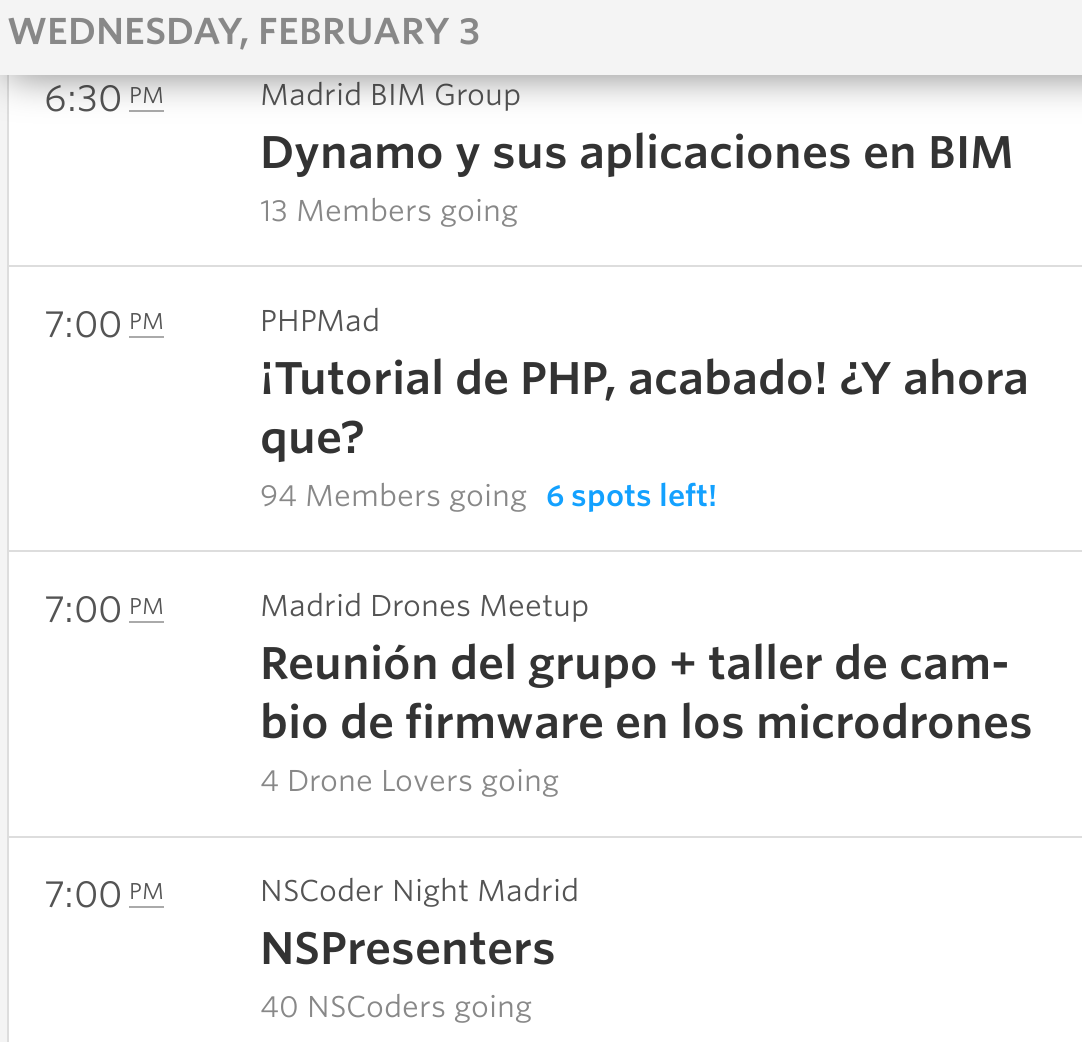
\includegraphics[width=6.5cm]{figs/meetup-calendar}

\begin{flushright}
  {\Large
    \url{http://meetup.com}
  }
\end{flushright}

\end{column}%
\hfill%
\begin{column}{.50\textwidth}
  \begin{flushright}
    
\includegraphics[width=5cm]{figs/meetup-logo}
  \end{flushright}
{\Large
\begin{itemize}
\item Información sobre reuniones cercanas
\item Mucho contenido ténico
\item Y mucho que no
\end{itemize}
}
\end{column}%
\end{columns}

\end{frame}

%%-----------------------------------------------------
\begin{frame}
\frametitle{Grupos}

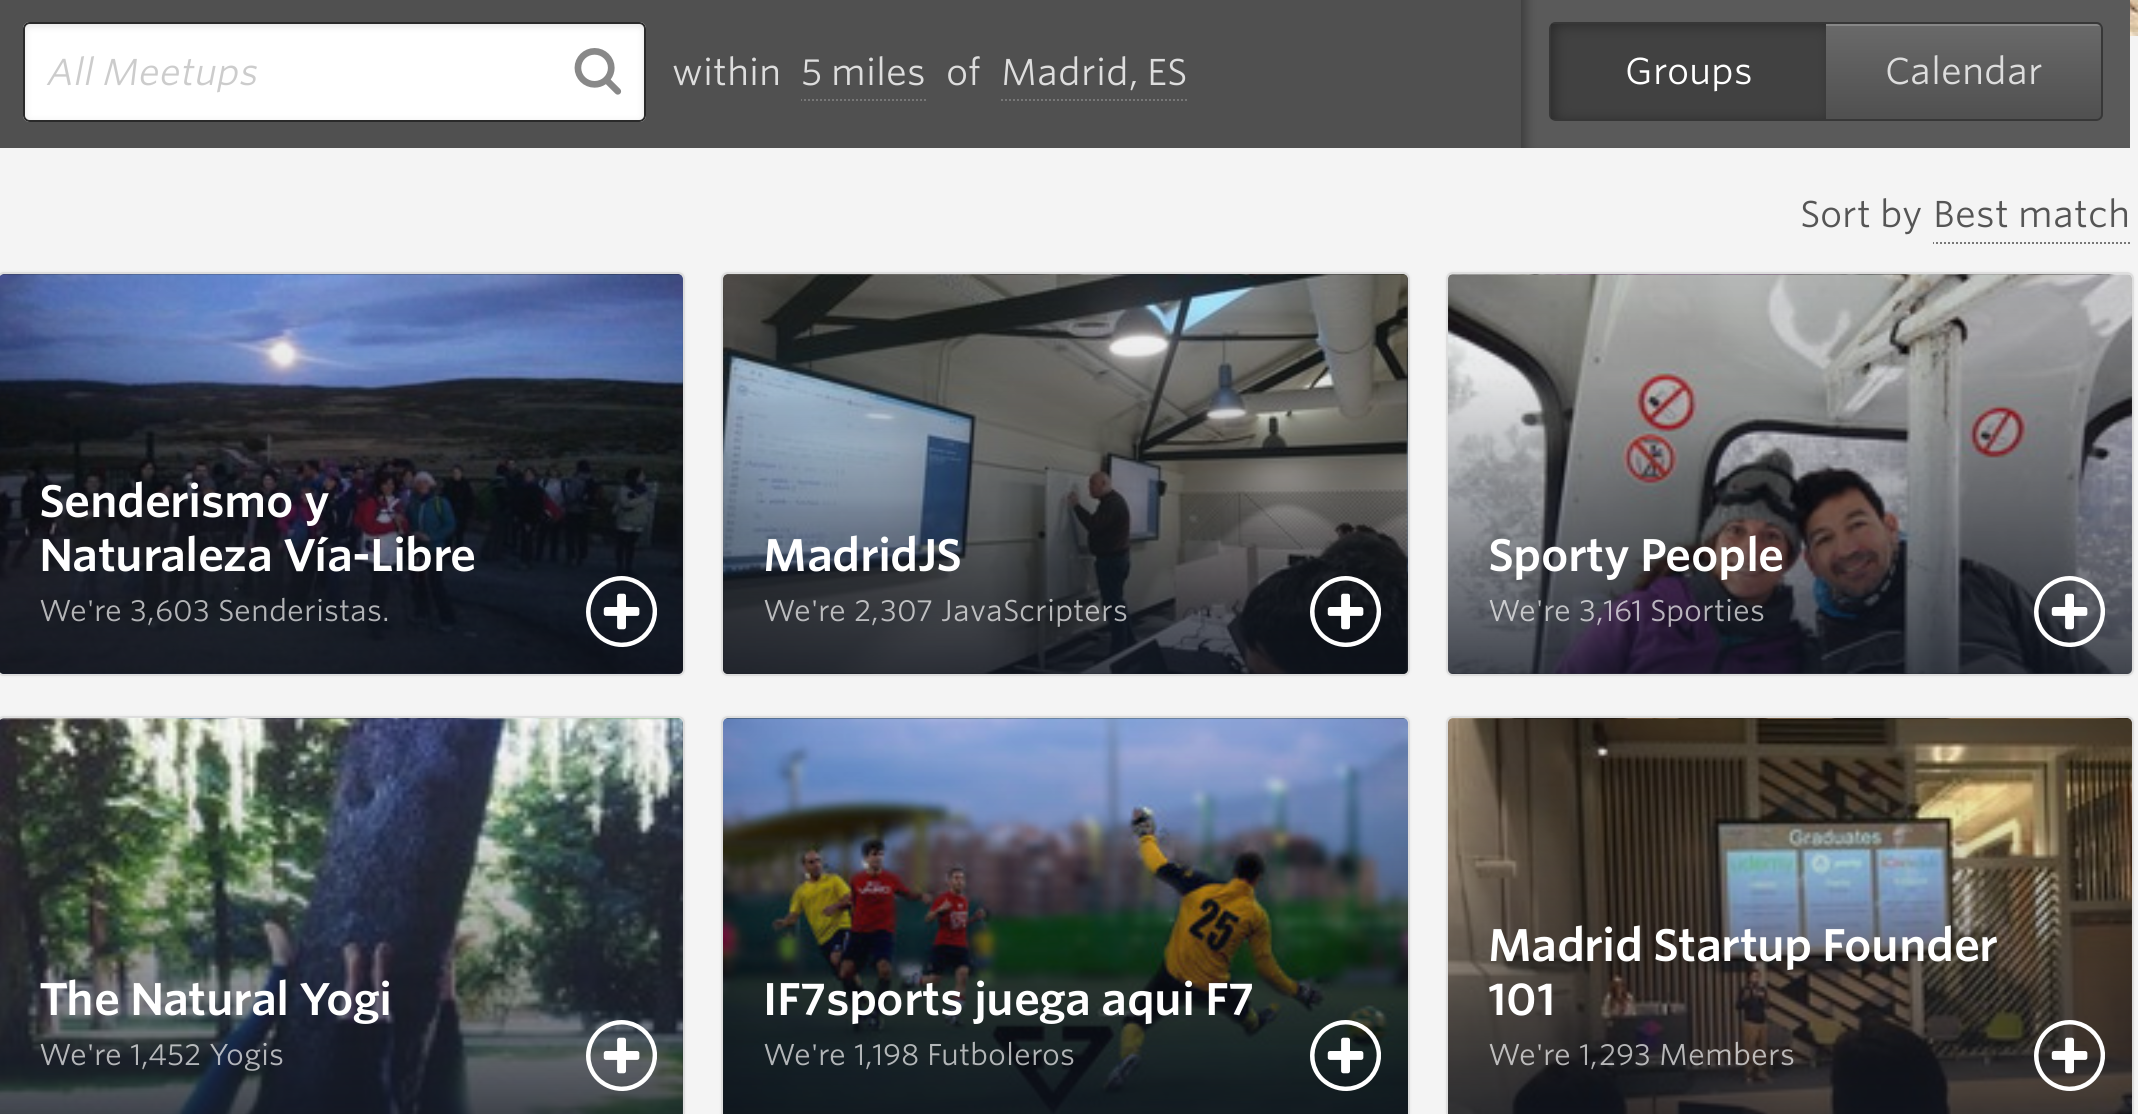
\includegraphics[width=11.5cm]{figs/meetup-near-madrid} 

\end{frame}

%%-----------------------------------------------------
\begin{frame}
\frametitle{Reuniones}

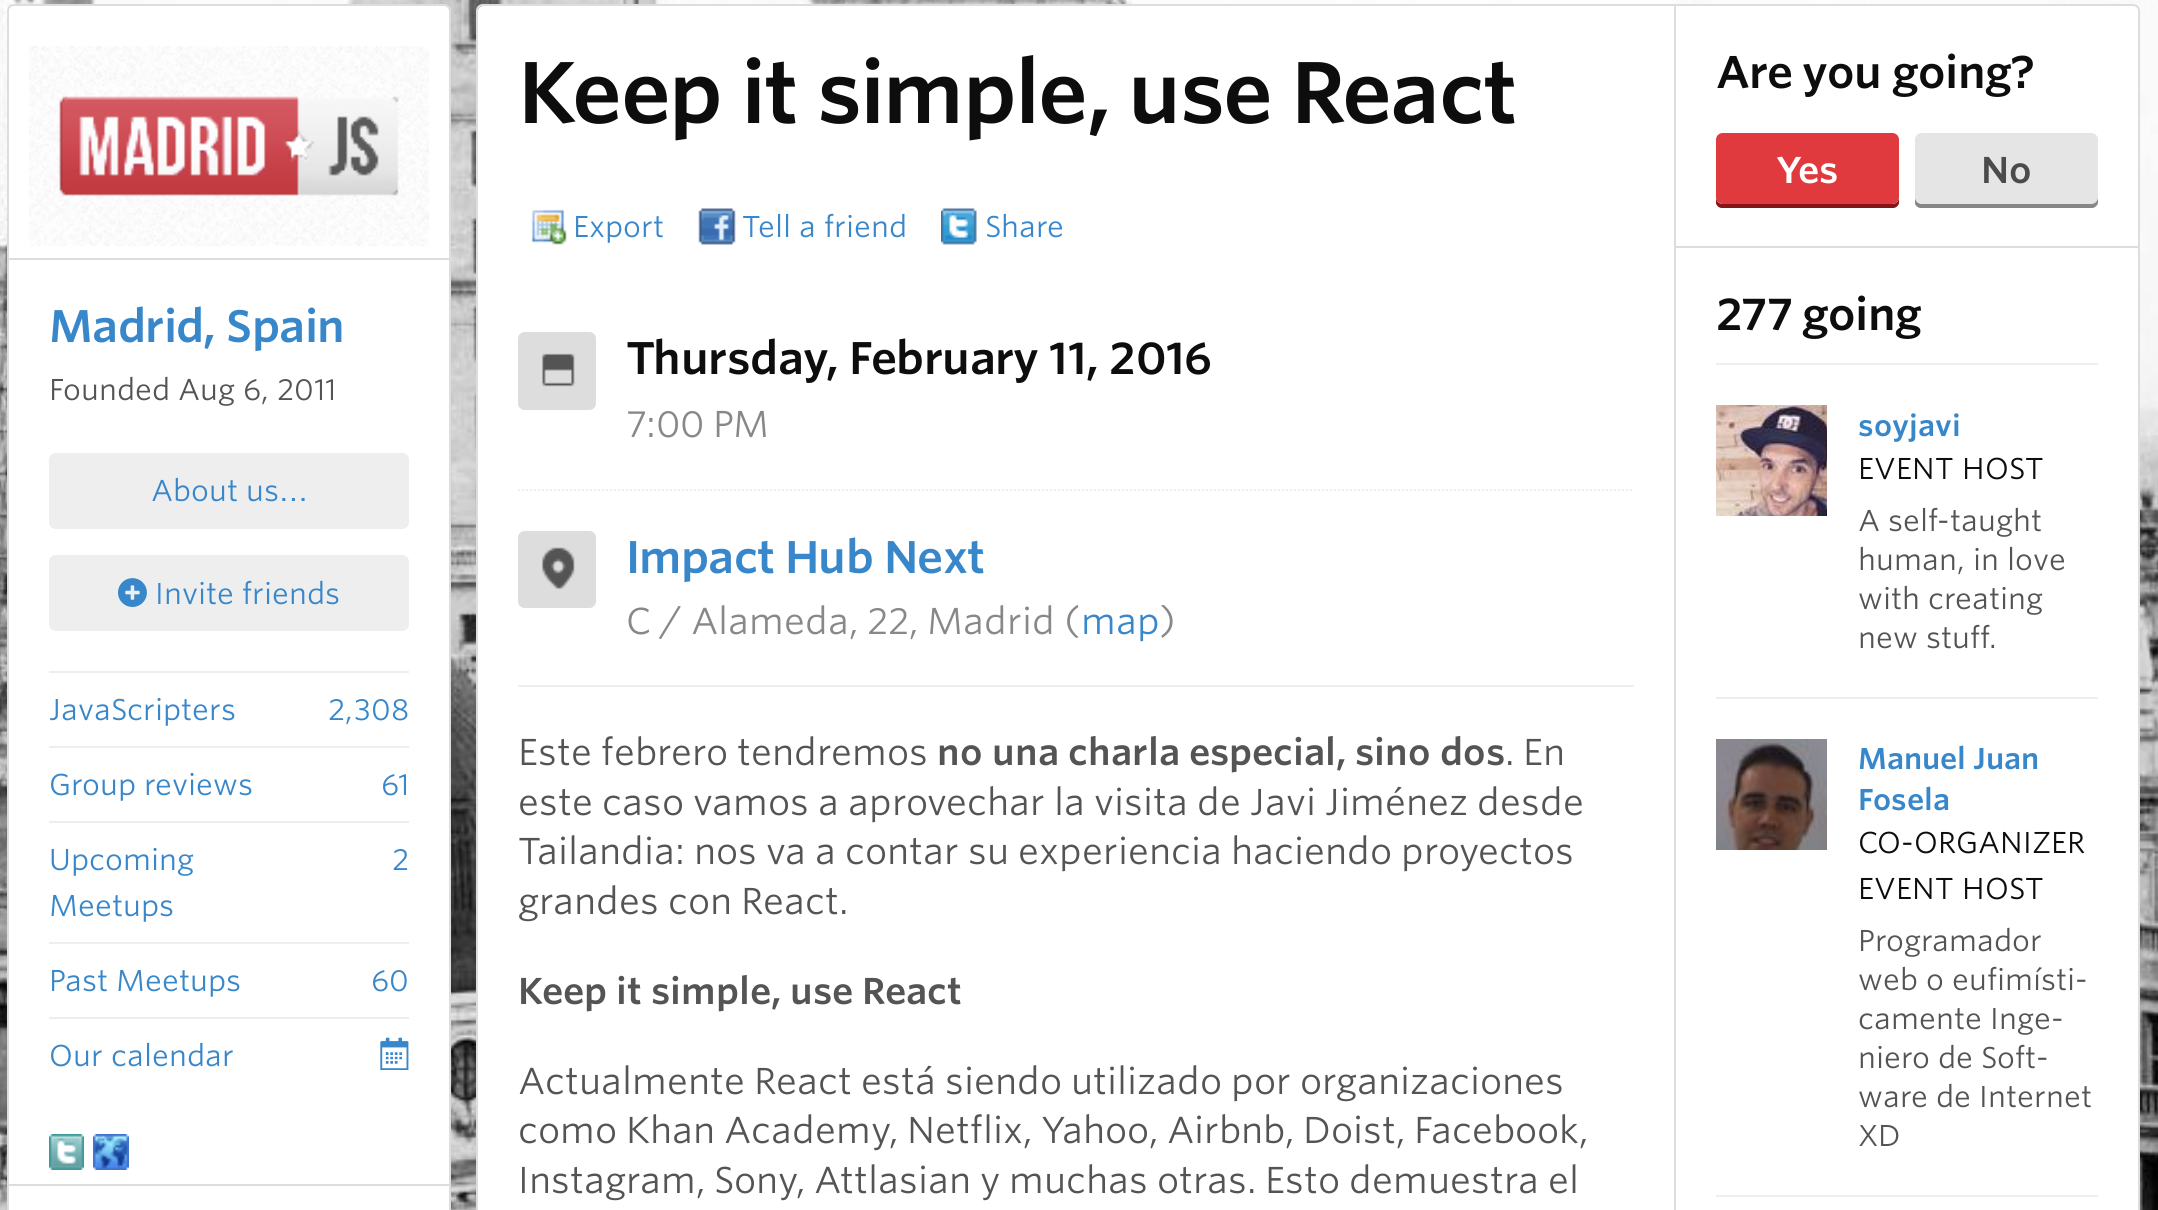
\includegraphics[width=11.5cm]{figs/meetup-meeting} 

\end{frame}






 % jgb

\end{document}
